\documentclass{article}

\usepackage{color}
\usepackage{mathrsfs,amsmath}
\usepackage{xcolor}
\usepackage{titlesec}
\usepackage{listings}
\usepackage{syntax}
\usepackage{fancyvrb}

\usepackage{graphicx}

\graphicspath{ {./assets/} }

\usepackage[margin=1.4in]{geometry}

\title{Balancer | Analysis} 
\author{Jared Dyreson}

\definecolor{mygray}{rgb}{0.4,0.4,0.4}
\definecolor{mygreen}{rgb}{0,0.8,0.6}
\definecolor{myorange}{rgb}{1.0,0.4,0}

\usepackage [english]{babel}
\usepackage [autostyle, english = american]{csquotes}
\MakeOuterQuote{"}

\titlespacing*{\section}
{0pt}{5.5ex plus 1ex minus .2ex}{4.3ex plus .2ex}
\titlespacing*{\subsection}
{0pt}{5.5ex plus 1ex minus .2ex}{4.3ex plus .2ex}

\usepackage{hyperref}
\hypersetup{
    colorlinks,
    citecolor=black,
    filecolor=black,
    linkcolor=black,
    urlcolor=black
}

\begin{document}

\maketitle
\tableofcontents

\newpage

\begin{abstract}
Current implementations of priority queues in the C++ Standard Template Library do not allow for on demand reordering.
Container objects are protected member attributes and cannot explicitly be modified.
This is a safety mechanism to not allow the user of the data structure to unintentionally break it.
However, since the goal is to bypass this, Balancer is a class that inherits from the base priority queue structure and provides this interface.
To still retain the original safety feature contained in the STL as only classes that are friends can request the data structure to reorder.
This also ensures that the structure cannot erratically change its state during the runtime of the program.
\end{abstract}

\section{Introduction}

\begin{flushleft}

This solution was provided by \href{https://stackoverflow.com/questions/5810190/how-to-tell-a-stdpriority-queue-to-refresh-its-ordering}{\underline{here}} by a user that suggested to inherit from the base std::priority_queue data structure.

\begin{figure}[!h]
\centering
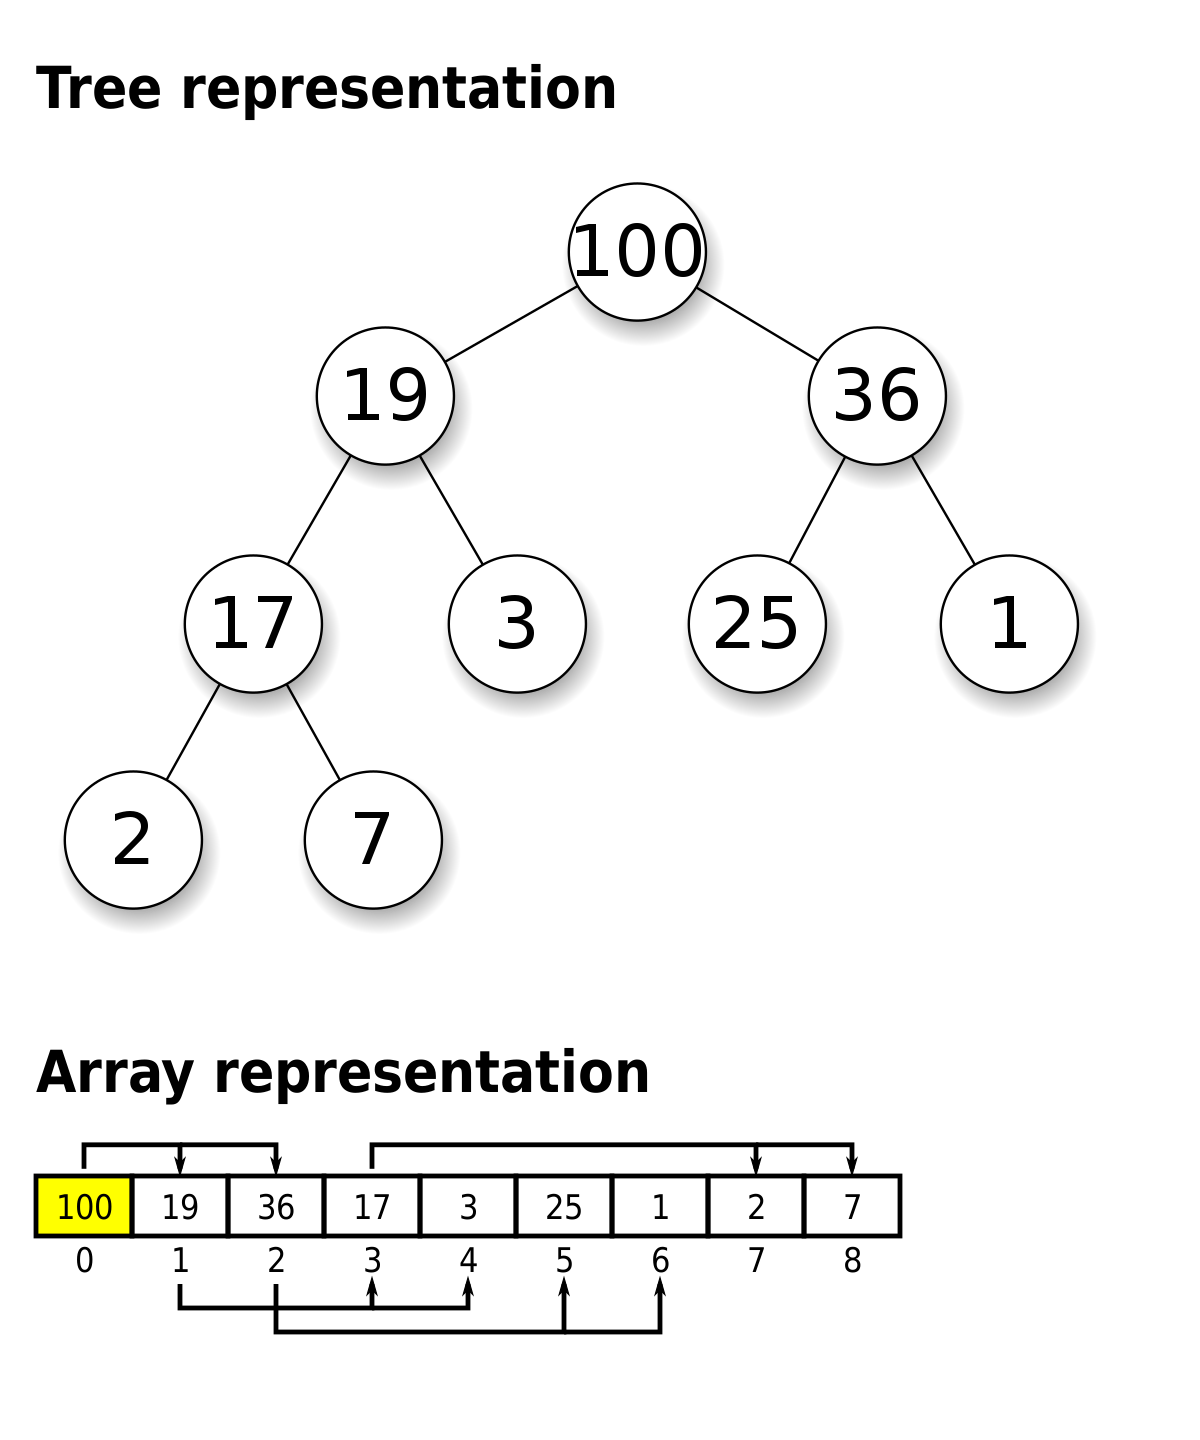
\includegraphics[width=5cm]{Max-Heap}
\caption{Example of Priority Heap}
\end{figure}

Priority queues with a special comparator function can influence how it's structured.
These functions can be customised to specific objects that are stored in the container.
In most use cases, node objects should have a time stamp object that indicates how old it is.
Older objects are generally assigned higher priority to avoid starvation.
\end{flushleft}

\newpage

\section{Use Cases}

\begin{flushleft}

Various types of programs can benefit from a reordering on demand paradigm.
CPU schedulers, fast food preparation and reservation systems could see an efficiency increase by using such a data structure.
All of these applications have some aspect of time that renders the tree stale.

\begin{figure}[!h]
\centering
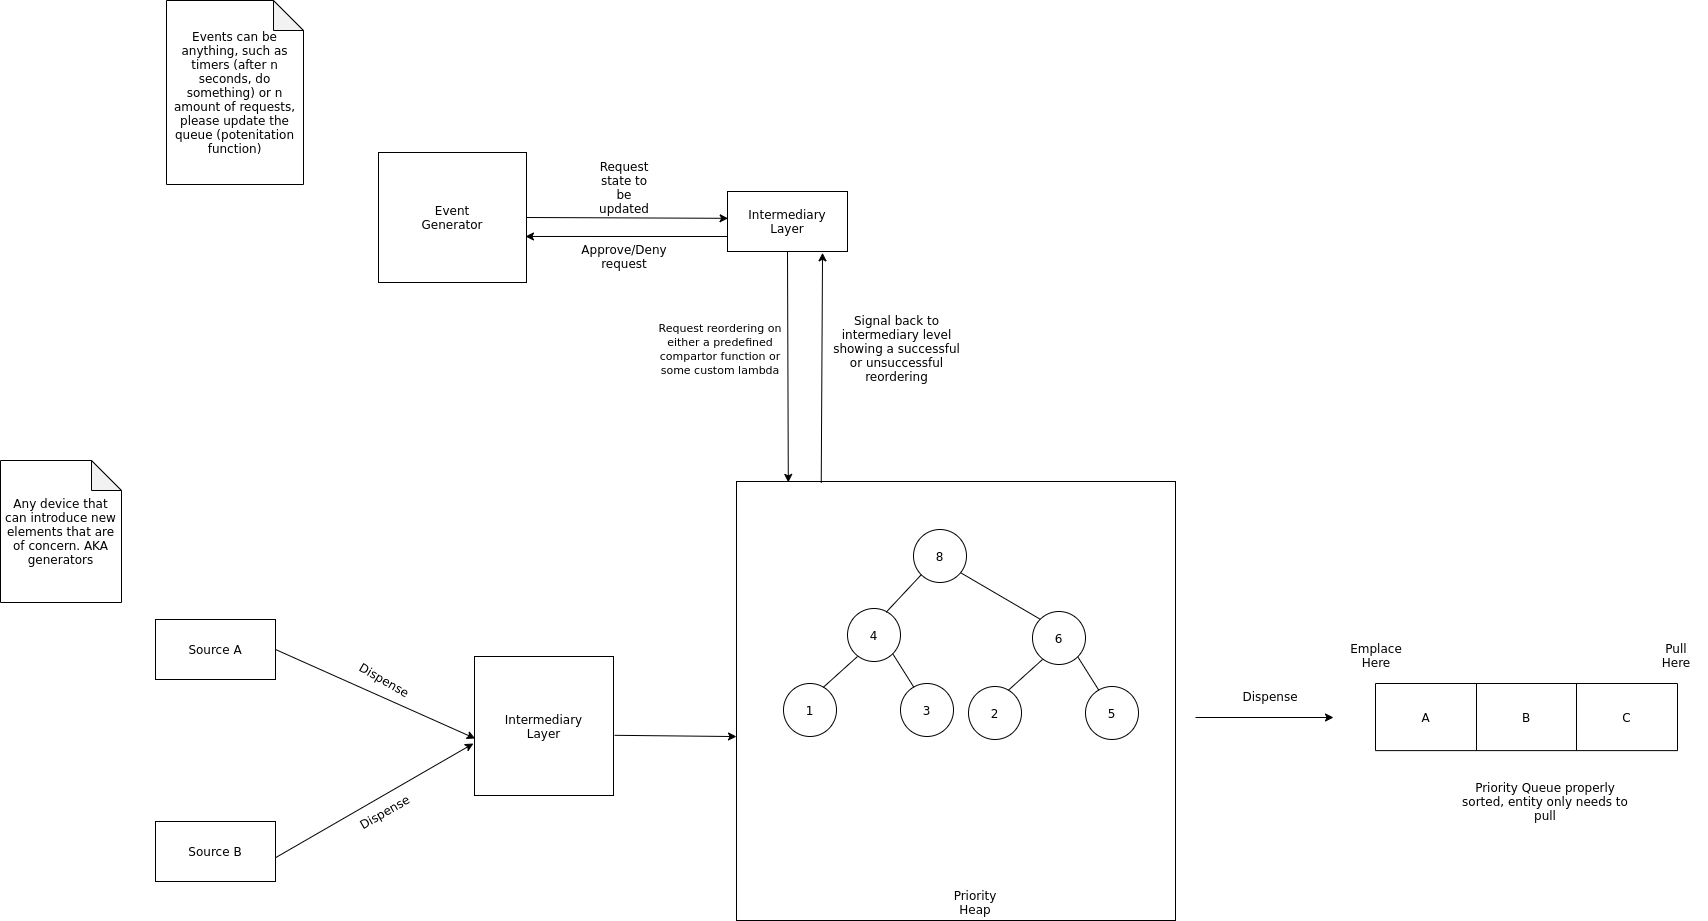
\includegraphics[width=15cm]{UseCaseSketch}
\caption{Example system}
\end{figure}

This sketch shows how the newly designed priority heap in action with respect to generalized inputs and outputs.
An arbitrary number of requests are spawned, which are then fed into another intermediary level that will funnel into the queue.
Upon insertion, the queue will reorder itself based on it's custom comparator function.
This still retains functionality from the original priority queue in STL, however also checks for the element's presence.
Some implementations can use a std::vector, however this checking process is $O(n)$ time, as all the elements would need to be evaluated.
We are also operating under the assumption that there is a potential for duplicate elements to be introduced into the system, which can stem from improper use of threads.
Please refer to the mathematical and algorithm analysis sections further down to get a more detailed explanation.

\end{flushleft}

\newpage

\section{Events}

Events are the only means of updating the state of the structure and are strictly outside influences to the system.
Timers are a common event which are outside the confines of the current system and can be implemented using std::thread_sleep.
More advanced events could measure the internal entropy of the system, such as the number of requests given or times the system reorders.
Such functions can be expressed using the following equation:
\[ 
		y_{k} = \phi \left( \sum_{j=0}^{m}w_{kj} \cdot x_{j} \right)
\]
$y_{k}$ denotes the strength of the output given by the inputs along with their respective weights.
Weights are used to signal how `important' an input is relative to others and can be generated using another outside algorithm.
For example, larger drink orders will hold a higher weight relative to smaller orders from another source.
The equation provided is the artificial neuron firing function, and it can be amended to fit this situation.
Once a predetermined threshold has been met, the system can then be prompted to reorder.
It is important to have a reasonable threshold because the system could reorder too frequently and diminish efficiency.

\section{Race Conditions}

One important factor to consider is how will the system operate when the heap is reorder.
A simple yet effective strategy is to apply a mutex over the resource, locking it from other processes that may wish to access the heap.
It is also necessary to note that this is another form of the Banker's Algorithm, wherein multiple processes are vying for resources.

\begin{figure}[!h]
\centering
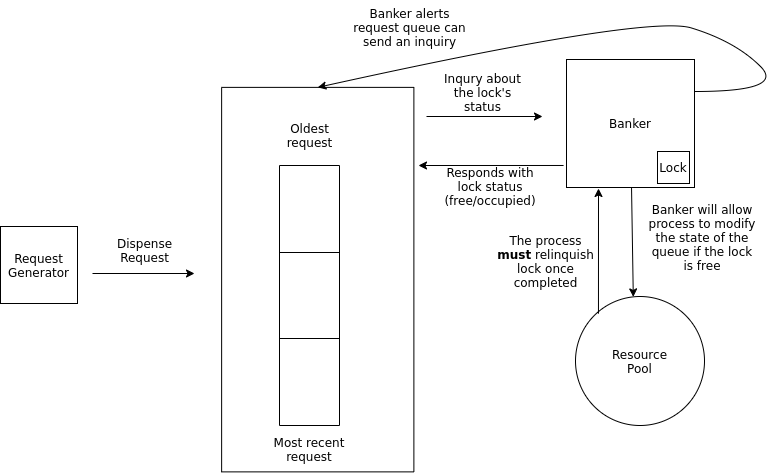
\includegraphics[width=9cm]{BankersAlgorithm}
\caption{Banker's Algorithm}
\end{figure}

An external class should manage the state of these processes and shall grant/deny requests.
Another approach would to shift the implementation to Rust, as it has a strong concurrency framework built into the language.
Further analysis needs to be conducted at a later date.

\newpage

\section{Algorithm and Mathematical Analysis}

\subsection{Reordering Algorithm | make_heap}

\subsubsection{Pseudocode}

\begin{verbatim}

function reorder {
      make_heap(underlying_container.begin, 
                underlying_container.end,
                comparator)
}
\end{verbatim}

\subsubsection{Mathematical Analysis}

\end{document}
